\documentclass[]{beamer}
\usepackage[utf8]{inputenc}
\usepackage{hyperref}
\usepackage{colortbl}
\usepackage{listings}
\lstset{
    basicstyle=\fontsize{10}{12}\selectfont\ttfamily,
    keywordstyle=\color{blue},         
    breaklines=true, 
    showtabs=false,
    showstringspaces=false,
    numberstyle=\tiny\color{mygray}
}
\usepackage{multirow}
\usepackage{pslatex}        % pour un pdf plus lisible à l'écran
%\usepackage{textcomp}

%\usetheme{AnnArbor}
%\usetheme{Antibes}
%\usetheme{Berkeley}
%\usetheme{Berlin}
%\usetheme{Boadilla}
\usetheme{CambridgeUS}
%\usetheme{Copenhagen}
%\usetheme{Dresden}
%\usetheme{Frankfurt}
%\usetheme{Goettingen}
%\usetheme{Hannover}
%\usetheme{JuanLesPins}
%\usetheme{Marburg}
%\usetheme{Montpellier}
%\usetheme{PaloAlto}
%\usetheme{Pittsburgh}
%\usetheme{Rochester}
%\usetheme{Singapore}
%\usetheme{Szeged}
%\usetheme{Warsaw}

% Force le plein écran
%\hypersetup{pdfpagemode=FullScreen}

% Barre de navigation
\setbeamertemplate{navigation symbols}{%
    \insertslidenavigationsymbol
    \insertframenavigationsymbol
    \insertsubsectionnavigationsymbol
    \insertsectionnavigationsymbol
    \insertdocnavigationsymbol
    \insertbackfindforwardnavigationsymbol
}


% contenu de la page de titre
\title[Demystifying some challenges from LCSC 2019]{Lëtz Cybersecurity Challenge 2019}
\subtitle{Demystifying some challenges}
\author{C\'{e}dric Bonhomme}
\institute[SMILE]{Security Made In Lëtzebuerg}
\date{March 09, 2019}
% \logo{\includegraphics[height=0.5cm]{./images/logo_crpht-soft.png}}
% Fin du préambule


\begin{document}
\begin{frame}
    \titlepage
\end{frame}


%
% SECTION: End of the presentation
%
\section*{What is this workshop about?}
\begin{frame}
    \frametitle{What is this workshop about?}
    \begin{center}
        \begin{itemize}
            \item we will present and deconstruct some challenges fron \href{https://github.com/cscluxembourg/vestatech}{LCSC 2019}.
        \end{itemize}
    \end{center}
\end{frame}


% --------- Sommaire ---------
\begin{frame}
    \frametitle{Contents}
    \tableofcontents
\end{frame}
% ----------------------------



%
% SECTION: Network analysis
%
\section{Network analysis}
\begin{frame}
    \frametitle{Contents}
    \begin{columns}[t]
        \begin{column}{5cm}
            \tableofcontents[sections={1-2}, currentsection, hideothersubsections]
        \end{column}
        \begin{column}{5cm}
            \tableofcontents[sections={3-4}, currentsection, hideothersubsections]
        \end{column}
    \end{columns}
\end{frame}
\subsection{Presentation and related challenges}
\begin{frame}
\frametitle{Presentation}
\framesubtitle{}

\end{frame}


\begin{frame}
\frametitle{Related challenge}
\begin{itemize}
    \item \href{https://github.com/cscluxembourg/vestatech/blob/master/challenges/find-the-author/gift.cap}{Find the author. The line was not secured.} - 1 star;
\end{itemize}
\bigskip
How did you solved this challenge?

\bigskip
From the feedbacks we got it seems that the majority of participants used Wireshark.
\end{frame}




\subsection{Tools}
\begin{frame}
\frametitle{}
\begin{itemize}
    \item tcpdump, BPF, Wireshark;
    \item little exercices with BPF filters, etc. solution of the challenge.
\end{itemize}
\end{frame}


\begin{frame}[fragile]
\frametitle{A pythonic solution}
\begin{lstlisting}[language=Python]
#! /usr/bin/python
# -*- coding: utf-8 -*-

# tcpflow -r gift.cap

with open("185.031.040.011.00080-010.008.000.006.37558" ,
            "r") as flow:
    data = flow.readlines()

for i, line in enumerate(data):
    if "Content-Type" in line:
        file_type = line.split("/")[1]
        with open("result", "w") as result:
            result.write("".join(data[i+1:]))
            exit()
\end{lstlisting}
\end{frame}
 


 

 
 

 
%
% SECTION: RSA
%
\section{A little cryptography with RSA}
\begin{frame}
    \frametitle{Contents}
    \begin{columns}[t]
        \begin{column}{5cm}
            \tableofcontents[sections={1-2}, currentsection, hideothersubsections]
        \end{column}
        \begin{column}{5cm}
            \tableofcontents[sections={3-4}, currentsection, hideothersubsections]
        \end{column}
    \end{columns}
\end{frame}
\subsection{Presentation and related challenges}
\begin{frame}
\frametitle{Presentation}
\begin{itemize}
    \item
\end{itemize}
\end{frame}

\begin{frame}
\frametitle{Related challenges}
\begin{itemize}
    \item \href{https://github.com/cscluxembourg/vestatech/blob/master/challenges/Sergei_forgot_his_formula/wip.py}{Sergei forgot his formula} - 2 stars;
    \item \href{https://github.com/cscluxembourg/vestatech/tree/master/challenges/A_key_from_the_past}{A key from the past} - 3 stars.
\end{itemize}
\bigskip
How did you solved these challenges?
\end{frame}

\begin{frame}
\frametitle{Related challenges - Sergei forgot his formula}
\begin{center}
    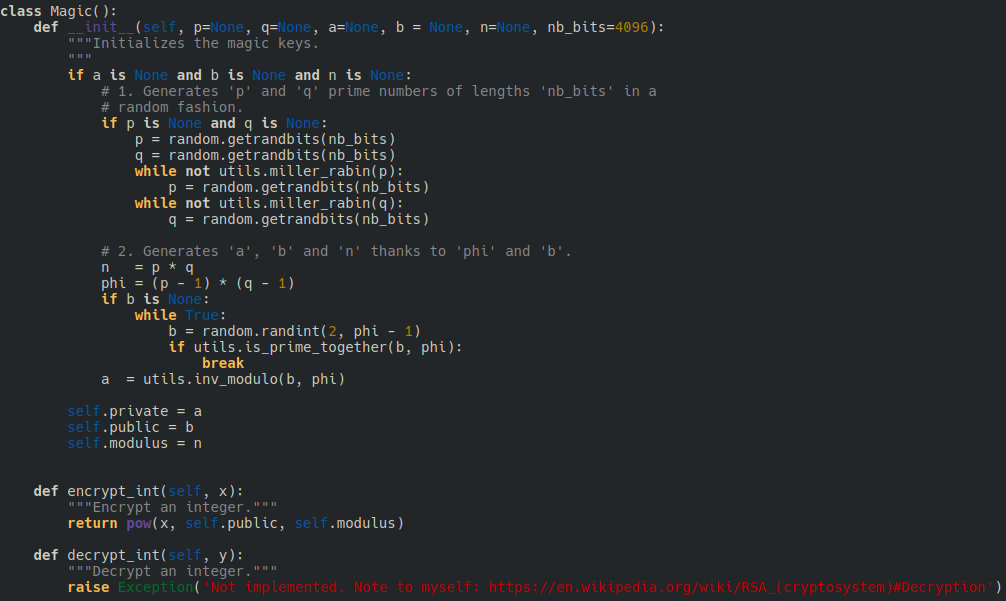
\includegraphics[height=6.5cm, width=12.0cm]{./images/RSA-algo-key-generation.png}
\end{center}
\href{https://en.wikipedia.org/wiki/RSA_(cryptosystem)\#Decryption}{Super easy} ;-)
\end{frame}


\begin{frame}
\frametitle{Related challenges - A key from the past}
\begin{center}
    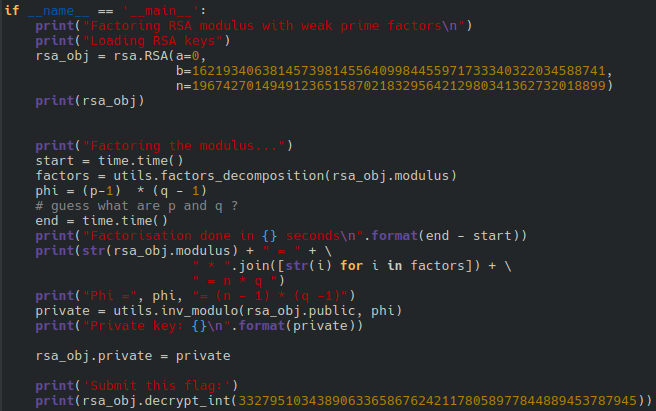
\includegraphics[height=6.5cm, width=12.0cm]{./images/RSA-weak-prime-factors.png}
\end{center}
\end{frame}




\subsection{Tools}



%
% SECTION: Steganography
%
\section{Steganography}
\begin{frame}
    \frametitle{Contents}
    \begin{columns}[t]
        \begin{column}{5cm}
            \tableofcontents[sections={1-2}, currentsection, hideothersubsections]
        \end{column}
        \begin{column}{5cm}
            \tableofcontents[sections={3-4}, currentsection, hideothersubsections]
        \end{column}
    \end{columns}
\end{frame}
\subsection{Presentation and related challenges}
\begin{frame}
\frametitle{What is steganography?}
\begin{itemize}
    \item steganography is the art and science of writing hidden messages in such a way that no one, apart from the sender and intended recipient, suspects the existence of the message, a form of security through obscurity.
    \item steganography is not cryptography.
\end{itemize}
\end{frame}

\begin{frame}
\frametitle{Related challenges}
\begin{itemize}
    \item \href{https://github.com/cscluxembourg/vestatech/blob/master/challenges/Vesta-asteroid/vesta.png}{Vesta asteroid} - 2 stars.
    \item \href{https://github.com/cscluxembourg/vestatech/blob/master/challenges/sergei/Sergei.png}{Sergei, our chief scientific officer} - 3 stars;
\end{itemize}
\bigskip
How did you solved these challenges?
\end{frame}

\begin{frame}
\frametitle{A picture can hide a lot of things...}
\begin{center}
    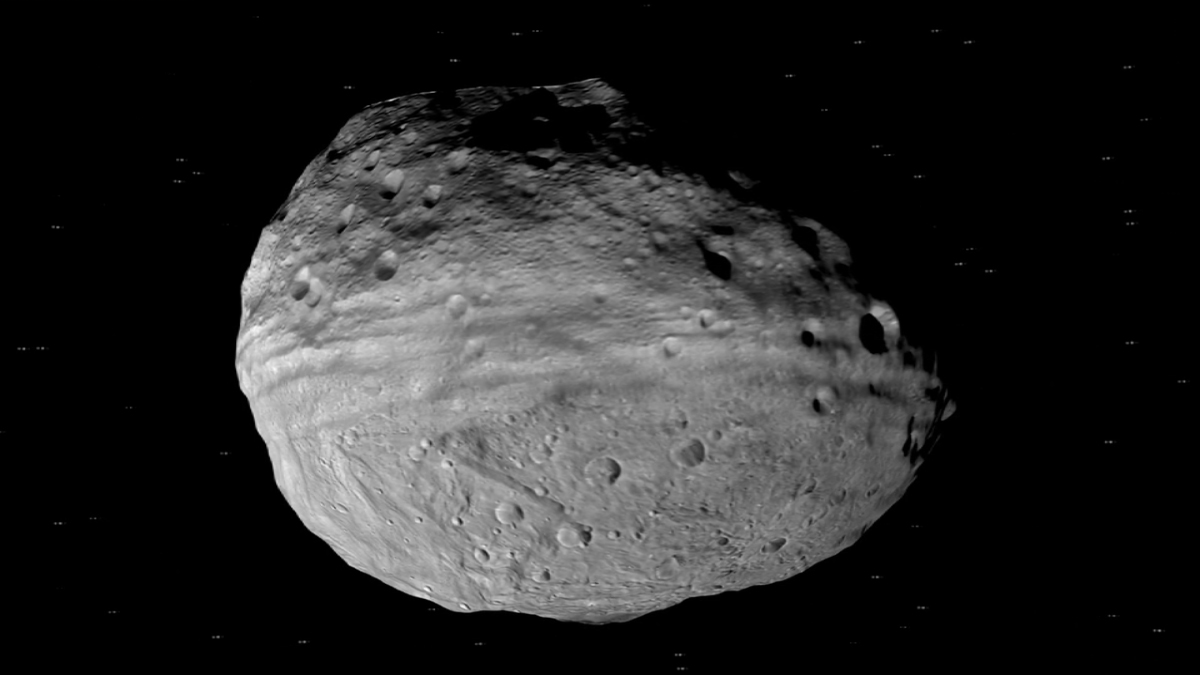
\includegraphics[height=6.0cm, width=12.0cm]{./images/vesta.png}
\end{center}
... thankfully, two gentle clues were placed on the VestaTech website.
\end{frame}

\begin{frame}
\frametitle{Detection - Parity steganalysis}
\begin{center}
    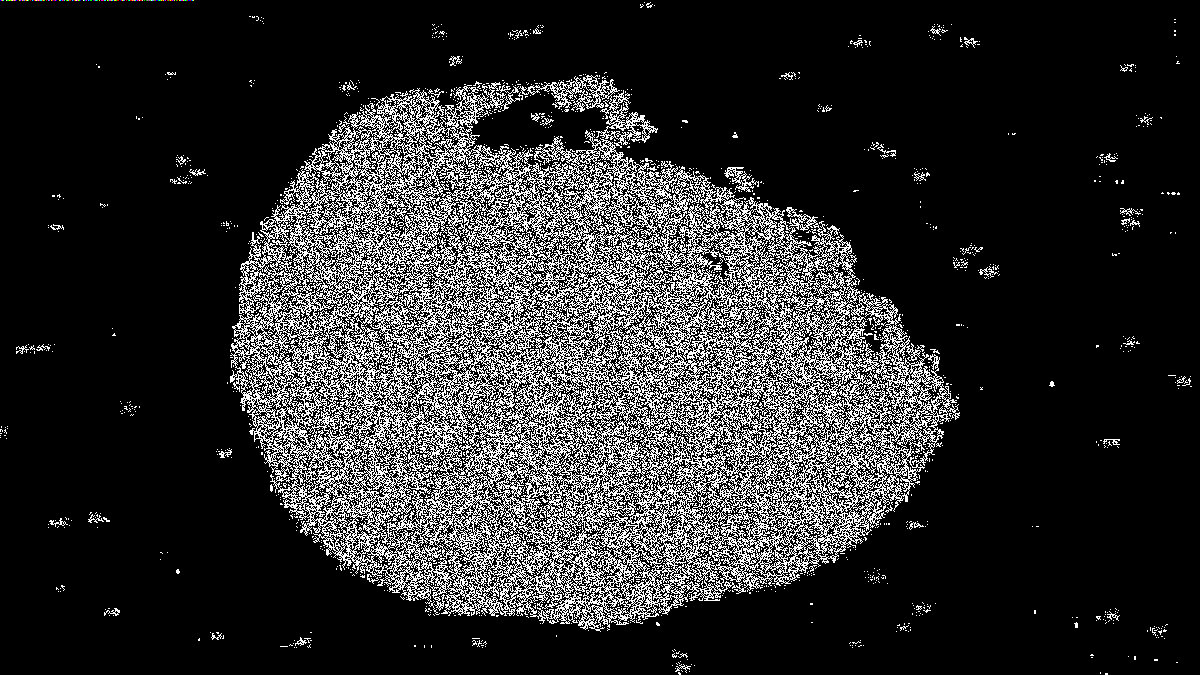
\includegraphics[height=6.0cm, width=12.0cm]{./images/vesta_steg.png}
\end{center}
Replace odd components by 255 and even by 0.

(132, 247, 123) $\longrightarrow$ (0, 255, 255)
\end{frame}

\begin{frame}
\frametitle{Detection - Parity steganalysis}
\begin{center}
    
\includegraphics[width=12.0cm]{./images/vesta_steg_zoom.png}
\end{center}
\end{frame}


\subsection{Tools}
\begin{frame}
\frametitle{}
\begin{itemize}
    \item \href{https://github.com/topics/steganography}{a lot of tools} are available;
\end{itemize}
\end{frame}

\begin{frame}[fragile]
\frametitle{A pythonic solution}
\begin{lstlisting}[language=Bash]
$ wget https://raw.githubusercontent.com/cscluxembourg/vestatech/master/challenges/sergei/Sergei.png
$ stegano-lsb reveal -i Sergei.png
$ stegano-lsb-set reveal -i Sergei.png -g fibonacci -s 9
\end{lstlisting}
\end{frame}




%
% SECTION: End of the presentation
%
\section*{End of the presentation}
\begin{frame}
    \frametitle{End of the presentation}
    \framesubtitle{Q and A}
    \begin{center}
        \begin{itemize}
            \item Thanks for listening.
            \item Any questions?
        \end{itemize}
    \end{center}
\end{frame}
\end{document}
